\documentclass{beamer}
\usetheme{Madrid}
\usecolortheme{dolphin}
\usepackage{amsmath}
\usepackage{graphicx}
\usepackage{tikz}
\usepackage{booktabs}

\title{Finite Difference Methods for Black-Scholes}
\subtitle{Numerical Solutions to Option Pricing PDEs}
\author{Lecturer}
\date{\today}

\begin{document}

\begin{frame}
\titlepage
\end{frame}

\begin{frame}
\frametitle{Outline}
\tableofcontents
\end{frame}

\section{Introduction to Finite Difference Methods}

\begin{frame}
\frametitle{The Black-Scholes PDE}
The Black-Scholes equation for option pricing is:

$$\frac{\partial V}{\partial t} + \frac{1}{2}\sigma^2 S^2 \frac{\partial^2 V}{\partial S^2} + rS \frac{\partial V}{\partial S} - rV = 0$$

\begin{itemize}
\item This parabolic PDE describes how option values evolve over time
\item Analytical solutions exist for simple cases (European options)
\item Complex options require numerical methods
\item Finite difference methods are powerful numerical techniques
\end{itemize}
\end{frame}

\begin{frame}
\frametitle{Why Use Finite Difference Methods?}
\begin{itemize}
\item \textbf{Analytical limitations}: Many option types lack closed-form solutions
\item \textbf{Complex boundaries}: American options, barrier options
\item \textbf{Variable parameters}: Time-dependent volatility, interest rates
\item \textbf{Multiple assets}: Basket options, spread options
\item \textbf{Flexibility}: Can handle various boundary conditions
\item \textbf{Accuracy}: Controlled approximation errors
\end{itemize}
\end{frame}

\section{Grid Construction and Discretization}

\begin{frame}
\frametitle{Computational Grid Setup}
Transform continuous PDE into discrete system:

\begin{columns}
\column{0.6\textwidth}
\textbf{Time dimension:}
\begin{itemize}
\item Divide $[0, T]$ into $N$ steps
\item Time step: $\Delta t = T/N$
\item Grid points: $t_j = j \cdot \Delta t$
\end{itemize}

\textbf{Price dimension:}
\begin{itemize}
\item Divide $[0, S_{\max}]$ into $M$ steps
\item Price step: $\Delta S = S_{\max}/M$
\item Grid points: $S_i = i \cdot \Delta S$
\end{itemize}

\column{0.4\textwidth}
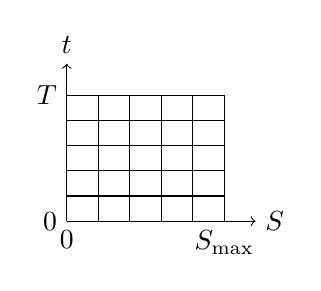
\begin{tikzpicture}[scale=0.8]
\draw[->] (0,0) -- (3,0) node[right] {$S$};
\draw[->] (0,0) -- (0,2.5) node[above] {$t$};
\foreach \x in {0,0.5,1,1.5,2,2.5} {
  \draw (\x,0) -- (\x,2);
}
\foreach \y in {0,0.4,0.8,1.2,1.6,2} {
  \draw (0,\y) -- (2.5,\y);
}
\node[below] at (0,0) {$0$};
\node[below] at (2.5,0) {$S_{\max}$};
\node[left] at (0,0) {$0$};
\node[left] at (0,2) {$T$};
\end{tikzpicture}
\end{columns}

\begin{block}{Grid Point Notation}
$V_{i,j} = V(S_i, t_j)$ represents option value at price $S_i$ and time $t_j$
\end{block}
\end{frame}

\begin{frame}
\frametitle{Finite Difference Approximations}
Replace continuous derivatives with discrete approximations:

\begin{block}{Time Derivative (Backward Difference)}
$$\frac{\partial V}{\partial t} \approx \frac{V_{i,j+1} - V_{i,j}}{\Delta t}$$
\end{block}

\begin{block}{First Price Derivative (Central Difference)}
$$\frac{\partial V}{\partial S} \approx \frac{V_{i+1,j} - V_{i-1,j}}{2\Delta S}$$
\end{block}

\begin{block}{Second Price Derivative (Central Difference)}
$$\frac{\partial^2 V}{\partial S^2} \approx \frac{V_{i+1,j} - 2V_{i,j} + V_{i-1,j}}{(\Delta S)^2}$$
\end{block}
\end{frame}

\section{Explicit Finite Difference Method}

\begin{frame}
\frametitle{Explicit Method Formulation}
Substitute finite difference approximations into Black-Scholes PDE:

$$\frac{V_{i,j+1} - V_{i,j}}{\Delta t} + \frac{1}{2}\sigma^2 S_i^2 \frac{V_{i+1,j} - 2V_{i,j} + V_{i-1,j}}{(\Delta S)^2}$$
$$+ rS_i \frac{V_{i+1,j} - V_{i-1,j}}{2\Delta S} - rV_{i,j} = 0$$

\begin{block}{Explicit Update Formula}
$$V_{i,j+1} = V_{i,j} + \Delta t \left[ -\frac{1}{2}\sigma^2 S_i^2 \frac{V_{i+1,j} - 2V_{i,j} + V_{i-1,j}}{(\Delta S)^2} - rS_i \frac{V_{i+1,j} - V_{i-1,j}}{2\Delta S} + rV_{i,j} \right]$$
\end{block}
\end{frame}

\begin{frame}
\frametitle{Explicit Method: Solution Procedure}
\begin{enumerate}
\item \textbf{Initialize boundary conditions}:
   \begin{itemize}
   \item At expiration: $V_{i,N} = \max(S_i - K, 0)$ for calls
   \item At price boundaries: appropriate conditions
   \end{itemize}

\item \textbf{Time stepping}: Work backward from expiration
   \begin{itemize}
   \item For $j = N-1, N-2, \ldots, 0$
   \item Update all interior points using explicit formula
   \end{itemize}

\item \textbf{Stability condition}: Must satisfy
   $$\Delta t \leq \frac{(\Delta S)^2}{\sigma^2 S_{\max}^2}$$
\end{enumerate}

\begin{block}{Advantages and Disadvantages}
\textbf{Pros}: Simple implementation, direct calculation\\
\textbf{Cons}: Stability restrictions, small time steps required
\end{block}
\end{frame}

\section{Implicit Finite Difference Method}

\begin{frame}
\frametitle{Implicit Method Formulation}
Use unknown values at time level $j+1$:

$$\frac{V_{i,j+1} - V_{i,j}}{\Delta t} + \frac{1}{2}\sigma^2 S_i^2 \frac{V_{i+1,j+1} - 2V_{i,j+1} + V_{i-1,j+1}}{(\Delta S)^2}$$
$$+ rS_i \frac{V_{i+1,j+1} - V_{i-1,j+1}}{2\Delta S} - rV_{i,j+1} = 0$$

\begin{block}{Matrix System}
This creates a system of linear equations at each time step:
$$\mathbf{A} \cdot \mathbf{V}^{j+1} = \mathbf{V}^j$$
where $\mathbf{A}$ is a tridiagonal matrix
\end{block}
\end{frame}

\begin{frame}
\frametitle{Implicit Method: Matrix Structure}
The coefficient matrix $\mathbf{A}$ has the form:

$$\mathbf{A} = \begin{pmatrix}
1+a_1 & b_1 & 0 & \cdots & 0 \\
c_2 & 1+a_2 & b_2 & \cdots & 0 \\
0 & c_3 & 1+a_3 & \cdots & 0 \\
\vdots & \vdots & \vdots & \ddots & \vdots \\
0 & 0 & 0 & \cdots & 1+a_M
\end{pmatrix}$$

where:
\begin{align}
a_i &= \Delta t \left( r + \frac{\sigma^2 S_i^2}{(\Delta S)^2} \right) \\
b_i &= -\frac{\Delta t}{2} \left( \frac{\sigma^2 S_i^2}{(\Delta S)^2} + \frac{rS_i}{\Delta S} \right) \\
c_i &= -\frac{\Delta t}{2} \left( \frac{\sigma^2 S_i^2}{(\Delta S)^2} - \frac{rS_i}{\Delta S} \right)
\end{align}
\end{frame}

\begin{frame}
\frametitle{Implicit Method: Advantages}
\begin{itemize}
\item \textbf{Unconditional stability}: No restrictions on time step size
\item \textbf{Larger time steps}: More efficient computation
\item \textbf{Better accuracy}: Often more accurate for given computational effort
\item \textbf{Robust}: Handles stiff problems well
\end{itemize}

\begin{block}{Solution Process}
\begin{enumerate}
\item Set up tridiagonal system at each time step
\item Solve using efficient algorithms (Thomas algorithm)
\item Work backward from expiration to present
\end{enumerate}
\end{block}

\begin{block}{Trade-off}
More complex implementation but superior numerical properties
\end{block}
\end{frame}

\section{Crank-Nicolson Method}

\begin{frame}
\frametitle{Crank-Nicolson: Best of Both Worlds}
Combines explicit and implicit methods using time-centered differences:

$$\frac{V_{i,j+1} - V_{i,j}}{\Delta t} + \frac{1}{2}\left[ \mathcal{L}V_{i,j} + \mathcal{L}V_{i,j+1} \right] = 0$$

where $\mathcal{L}$ is the spatial differential operator:
$$\mathcal{L}V = \frac{1}{2}\sigma^2 S^2 \frac{\partial^2 V}{\partial S^2} + rS \frac{\partial V}{\partial S} - rV$$

\begin{block}{Key Properties}
\begin{itemize}
\item \textbf{Second-order accurate} in both time and space
\item \textbf{Unconditionally stable}
\item \textbf{Most commonly used} in practice
\end{itemize}
\end{block}
\end{frame}

\begin{frame}
\frametitle{Crank-Nicolson Implementation}
The discretized equation becomes:

$$\left( \mathbf{I} - \frac{\Delta t}{2}\mathbf{L} \right) \mathbf{V}^{j+1} = \left( \mathbf{I} + \frac{\Delta t}{2}\mathbf{L} \right) \mathbf{V}^j$$

where $\mathbf{L}$ is the discretized spatial operator matrix.

\begin{block}{Solution Algorithm}
\begin{enumerate}
\item Form matrices $\mathbf{A} = \mathbf{I} - \frac{\Delta t}{2}\mathbf{L}$ and $\mathbf{B} = \mathbf{I} + \frac{\Delta t}{2}\mathbf{L}$
\item At each time step: solve $\mathbf{A} \mathbf{V}^{j+1} = \mathbf{B} \mathbf{V}^j$
\item Use efficient tridiagonal solvers
\end{enumerate}
\end{block}

\textbf{Result}: Optimal balance of accuracy, stability, and efficiency
\end{frame}

\section{Boundary Conditions}

\begin{frame}
\frametitle{Essential: Proper Boundary Conditions}
Boundary conditions are crucial for accurate solutions:

\begin{columns}
\column{0.5\textwidth}
\textbf{European Call Options:}
\begin{itemize}
\item At $S = 0$: $V(0,t) = 0$
\item At $S = S_{\max}$: \\$V(S_{\max},t) = S_{\max} - Ke^{-r(T-t)}$
\item At $t = T$: \\$V(S,T) = \max(S-K, 0)$
\end{itemize}

\column{0.5\textwidth}
\textbf{European Put Options:}
\begin{itemize}
\item At $S = 0$: $V(0,t) = Ke^{-r(T-t)}$
\item At $S = S_{\max}$: $V(S_{\max},t) = 0$
\item At $t = T$: \\$V(S,T) = \max(K-S, 0)$
\end{itemize}
\end{columns}

\begin{block}{Implementation Notes}
\begin{itemize}
\item Choose $S_{\max}$ large enough so boundary effects are negligible
\item Ensure boundary conditions are consistent with PDE
\item Handle corner points carefully
\end{itemize}
\end{block}
\end{frame}

\end{document}